\chapter{2-Layered Architecture}
\label{ch:2_layered}

The 2-layered architecture is a practical starting point for student projects and smaller systems. We separate software into a \textit{presentation} layer and a \textit{persistence} layer, so we can keep responsibilities visible from the beginning.

In this chapter, we start with this minimal shape and then evolve it by introducing entities as a dedicated module. This gives us a bridge from simple layered systems toward richer architectural styles.

\section{Why We Start with Two Layers}
\label{sec:2_layered_why}

When we begin with architecture, we usually want structure without too much ceremony. Two layers give us that balance:
\begin{itemize}
    \item the presentation layer handles user interaction and application actions,
    \item the persistence layer stores and retrieves entities.
\end{itemize}

For simple systems, this is often enough. We can move quickly, keep code easy to explain, and still establish separation of concerns from day one.

\section{Initial Shape: Presentation and Persistence}
\label{sec:2_layered_initial_shape}

The initial form contains two modules with one main dependency direction: presentation depends on persistence to load and store data.

\begin{figure}[htbp]
    \centering
    \usetikzlibrary{arrows.meta, positioning}

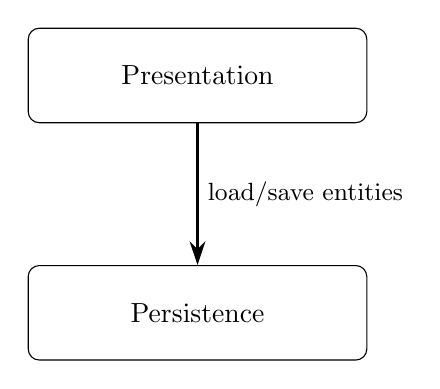
\begin{tikzpicture}[
    node distance=1.8cm,
    module/.style={draw, rounded corners, minimum width=4.3cm, minimum height=1.2cm, align=center},
    dep/.style={-{Stealth[length=3mm, width=2mm]}, thick}
]
    \node[module] (presentation) {Presentation};
    \node[module, below=of presentation] (persistence) {Persistence};

    \draw[dep] (presentation.south) -- node[right, font=\small] {load/save entities} (persistence.north);
\end{tikzpicture}

    \caption{Initial 2-layered shape with presentation and persistence.}
    \label{fig:2_layered_initial_shape}
\end{figure}

\subsection{Presentation Layer Responsibilities}
\label{sec:2_layered_presentation_responsibilities}

The presentation layer coordinates incoming interaction and triggers application actions. In practice, this can be:
\begin{itemize}
    \item a JavaFX controller responding to button clicks and form events,
    \item or a Web API controller responding to HTTP requests.
\end{itemize}

In both cases, we parse input, call the relevant action, and prepare output for the user interface or API response.

\subsection{Persistence Layer Responsibilities}
\label{sec:2_layered_persistence_responsibilities}

The persistence layer has one core responsibility: \textbf{persist entities}. It saves and retrieves domain data (for example \texttt{Kaiju} and \texttt{Breach}) using a storage technology such as a database.

This layer should focus on persistence concerns such as queries, mapping, and transaction boundaries. It should not contain user-interface behavior.

\subsection{Java Example from the Presentation Layer}
\label{sec:2_layered_javafx_example}

We start with JavaFX as the primary example because many student systems begin with a desktop GUI.

\needspace{24\baselineskip}
\begin{ridercode}{Java}
public final class ConfirmDetectionController {
    private final KaijuRepository kaijuRepository;
    private final BreachRepository breachRepository;

    public ConfirmDetectionController(KaijuRepository kaijuRepository,
                                      BreachRepository breachRepository) {
        this.kaijuRepository = kaijuRepository;
        this.breachRepository = breachRepository;
    }

    public void onConfirmDetection(String codename,
                                   String classification,
                                   String breachId) {
        Breach breach = breachRepository.loadById(breachId)
                .orElseThrow(() -> new IllegalArgumentException("Unknown breach"));

        Kaiju kaiju = Kaiju.confirmed(codename, classification, breach.id());
        kaijuRepository.save(kaiju);
    }
}
\end{ridercode}

The same responsibility can also be implemented in a Web API controller. The transport changes, but the intent remains the same: receive input, perform the action, and persist entities through persistence interfaces.

\section{Step 2: Introduce Entities as a New Module}
\label{sec:2_layered_step2_entities}

As systems grow, we usually discover that both presentation and persistence rely on the same domain concepts. At that point, we can introduce \texttt{entities} as a dedicated module and move shared domain types there.

\begin{figure}[htbp]
    \centering
    \usetikzlibrary{arrows.meta, positioning}

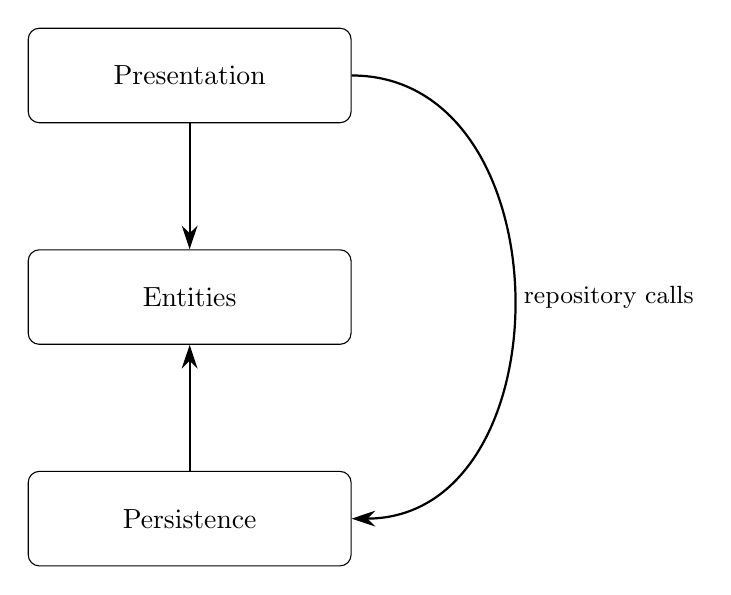
\begin{tikzpicture}[
    node distance=1.6cm and 1.8cm,
    module/.style={draw, rounded corners, minimum width=4.1cm, minimum height=1.2cm, align=center},
    dep/.style={-{Stealth[length=3mm, width=2mm]}, thick}
]
    \node[module] (presentation) {Presentation};
    \node[module, below=of presentation] (entities) {Entities};
    \node[module, below=of entities] (persistence) {Persistence};

    \draw[dep] (presentation.south) -- (entities.north);
    \draw[dep] (presentation.east) to[out=0, in=0, looseness=1.25] node[right, font=\small] {repository calls} (persistence.east);
    \draw[dep] (persistence.north) -- (entities.south);
\end{tikzpicture}

    \caption{Evolved structure with entities as a separate module.}
    \label{fig:2_layered_with_entities}
\end{figure}

\subsection{Why Entities Move Out of Persistence}
\label{sec:2_layered_why_entities_module}

Entities represent business concepts, not storage technology. For example, \texttt{Kaiju}, \texttt{Breach}, and related identifiers are part of domain meaning used across the system.

By placing entities in their own module:
\begin{itemize}
    \item presentation can work with domain concepts directly,
    \item persistence can map those concepts to storage models,
    \item and entities remain independent of GUI or database details.
\end{itemize}

\subsection{Updated Dependency Rules}
\label{sec:2_layered_dependency_rules}

After adding the entities module, dependency direction should stay explicit:
\begin{itemize}
    \item \texttt{presentation} may depend on \texttt{entities} and persistence contracts,
    \item \texttt{persistence} may depend on \texttt{entities},
    \item \texttt{entities} should not depend on \texttt{presentation} or \texttt{persistence}.
\end{itemize}

\begin{figure}[htbp]
    \centering
    \usetikzlibrary{arrows.meta, positioning}

\begin{tikzpicture}[
    node distance=2.0cm and 2.0cm,
    module/.style={draw, rounded corners, minimum width=4.2cm, minimum height=1.2cm, align=center},
    dep/.style={-{Stealth[length=3mm, width=2mm]}, thick}
]
    \node[module] (presentation) {Presentation};
    \node[module, right=of presentation] (persistence) {Persistence};
    \node[module, below=of $(presentation)!0.5!(persistence)$] (entities) {Entities};

    \draw[dep] (presentation.south) -- node[left, font=\small] {uses} (entities.north west);
    \draw[dep] (persistence.south) -- node[right, font=\small] {maps to/from} (entities.north east);
    \draw[dep] (presentation.east) -- node[above, font=\small] {calls persistence} (persistence.west);
\end{tikzpicture}

    \caption{Dependency direction after introducing entities.}
    \label{fig:2_layered_dependency_rules}
\end{figure}

\section{Where Business Logic Goes in This Style}
\label{sec:2_layered_logic_placement}

In this architecture level, when business logic starts to appear, we keep it in presentation actions or controller methods (JavaFX or Web API controllers). That keeps the design straightforward while systems are still small.

For example, validation and simple coordination can remain in methods like \texttt{onConfirmDetection(...)} or a REST action method. If this logic becomes large, duplicated, or difficult to test, that is a signal to evolve the architecture further.

\subsection{Where the Logic Lives}
\label{sec:2_layered_where_logic_lives}

In this setup, the controller is no longer only a traffic cop routing requests. It becomes the practical execution center for each action. This is a deliberate simplification for small systems.

In a Web API controller method, we may receive the HTTP request, validate incoming data, perform a calculation or business rule check, and then persist through a repository or ORM call in one place.

In JavaFX, an \texttt{onButtonClick(...)} handler may do the same: validate form input, calculate totals or taxes, and save the resulting entity to the database through the persistence layer.

\begin{figure}[htbp]
    \centering
    \usetikzlibrary{arrows.meta, positioning}

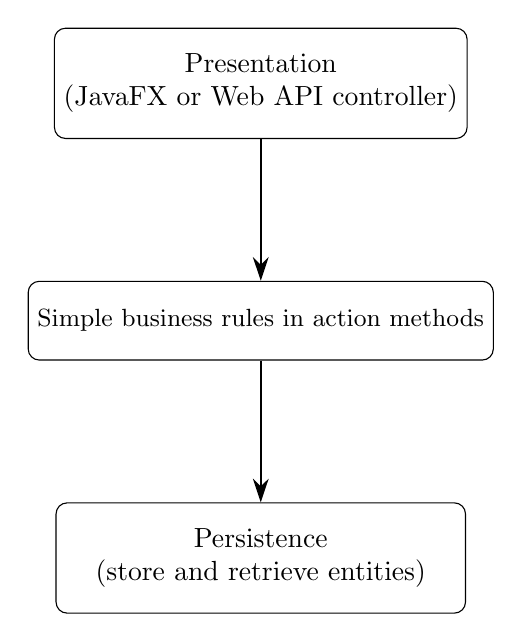
\begin{tikzpicture}[
    node distance=1.8cm and 2.4cm,
    module/.style={draw, rounded corners, minimum width=5.2cm, minimum height=1.4cm, align=center},
    note/.style={draw, rounded corners, minimum width=5.2cm, minimum height=1.0cm, align=center, font=\small},
    dep/.style={-{Stealth[length=3mm, width=2mm]}, thick}
]
    \node[module] (presentation) {Presentation\\(JavaFX or Web API controller)};
    \node[note, below=of presentation] (logic) {Simple business rules in action methods};
    \node[module, below=of logic] (persistence) {Persistence\\(store and retrieve entities)};

    \draw[dep] (presentation.south) -- (logic.north);
    \draw[dep] (logic.south) -- (persistence.north);
\end{tikzpicture}

    \caption{Business logic placement for the 2-layered approach.}
    \label{fig:2_layered_logic_placement}
\end{figure}

\subsection{Signs You Are Outgrowing the Style}
\label{sec:2_layered_outgrowing}

This architecture works best for simple systems. We should consider a richer style when we see repeated symptoms:
\begin{itemize}
    \item controller methods become very long and hard to reason about,
    \item the same business rules appear in multiple controllers,
    \item persistence concerns leak into presentation code,
    \item tests become slow because most behavior requires full-stack execution.
\end{itemize}

\section{Testing Strategy for Two Layers}
\label{sec:2_layered_testing}

A practical testing strategy for this style is:
\begin{itemize}
    \item test controller actions with mocked or fake repositories,
    \item test persistence adapters with focused integration tests,
    \item keep end-to-end tests for key user flows only.
\end{itemize}

This gives us fast feedback while still validating that data persistence works against real infrastructure.

\section{Practical Trade-offs}
\label{sec:2_layered_tradeoffs}

The 2-layered approach gives us speed and clarity early on, but it is intentionally limited.\autocite{fowler2002patterns}

\subsection{Pros: The Simpler Side}
\label{sec:2_layered_pros}

\begin{itemize}
    \item \textbf{Speed:} we can build features quickly because there are fewer layers and fewer files to traverse.
    \item \textbf{Less mapping ceremony:} we often avoid extra translation steps between multiple architectural layers.
    \item \textbf{Lower learning curve:} this is approachable for junior students and useful for early project phases.
\end{itemize}

\subsection{Cons: The Mixed-Concerns Side}
\label{sec:2_layered_cons}

\begin{itemize}
    \item \textbf{Fat controllers:} single action methods can grow very large and become hard to read.
    \item \textbf{Duplication risk:} if the same rule is needed in Web API, UI, and jobs, copy-paste is common.
    \item \textbf{Harder isolated testing:} logic tied to controller flows is harder to test without framework setup.
    \item \textbf{Mixed concerns:} transport and business concerns can become tightly interwoven.
\end{itemize}

\subsection{The Leaky Abstraction Problem}
\label{sec:2_layered_leaky_abstraction}

The biggest structural risk is framework coupling. If business logic lives directly in controller methods, that logic can become tied to framework objects and conventions, such as HTTP request/response types or JavaFX event handling APIs.

As a result, moving the same behavior to a different delivery mechanism (for example from JavaFX to Web UI, or from Web API to CLI) may require extraction and rewrite work instead of simple reuse.

\subsection{When 2-Layer Is Actually Okay}
\label{sec:2_layered_when_okay}

Two layers can be the right choice when the solution space is genuinely small. This is consistent with Fowler's \textit{Transaction Script} style,\autocite{fowler2002patterns} where simple request-like actions execute straightforward logic directly.

\begin{itemize}
    \item simple CRUD workflows with low rule complexity,
    \item short-lived prototypes or throwaway internal tools,
    \item very small services with narrow and stable behavior.
\end{itemize}

\subsection{The Slippery Slope}
\label{sec:2_layered_slippery_slope}

The danger is that systems rarely stay simple forever. A small tool can become mission-critical, and by then controllers may already be large and tightly coupled.

When that happens, extracting logic into clearer architectural boundaries becomes expensive. This is why we treat 2-layered architecture as a practical starting point and watch carefully for growth signals.

\begin{figure}[htbp]
    \centering
    \usetikzlibrary{arrows.meta, positioning}

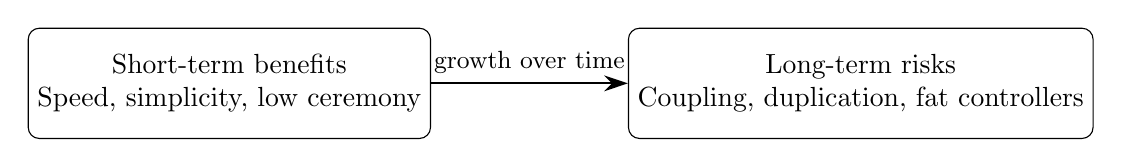
\begin{tikzpicture}[
    node distance=2.0cm and 2.5cm,
    box/.style={draw, rounded corners, align=center, minimum width=4.8cm, minimum height=1.4cm},
    arrow/.style={-{Stealth[length=3mm, width=2mm]}, thick}
]
    \node[box] (pros) {Short-term benefits\\Speed, simplicity, low ceremony};
    \node[box, right=of pros] (cons) {Long-term risks\\Coupling, duplication, fat controllers};

    \draw[arrow] (pros.east) -- node[above, font=\small] {growth over time} (cons.west);
\end{tikzpicture}

    \caption{Trade-off balance in 2-layered architecture: short-term speed versus long-term coupling risk.}
    \label{fig:2_layered_tradeoffs_balance}
\end{figure}

In short, we use this architecture as a teaching baseline and a valid production option for simple systems. When complexity rises, it becomes a stepping stone toward stronger separation of behavior and infrastructure.
